\chapter{Analisi di robustezza}
\label{chap:analisi-robustezza}
In questo capitolo presenteremo una tecnica per valutare della robustezza delle
implementazioni del protocollo proposto. L'obiettivo è quello di trovare
la probabilità $ R_c $ che il segreto venga pubblicato una volta raggiunta la deadline
(requisito di \hyperref[parag:certezza-pubblicazione]{\textit{certezza di pubblicazione}})
e la probabilità $ R_s $ che il messaggio rimanga segreto fino alla deadline
(requisito di \hyperref[parag:segretezza-tre]{\textit{segretezza del messaggio}}).

\section{Terminologia}

\paragraph{Numero di share}
Il numero di share $ n $ è uno dei parametri
dell'algoritmo di secret sharing, utilizzato dalla versione
avanzata del protocollo.
Facciamo notare che la versione base può essere vista come un caso particolare
della versione avanzata, dove $ n = 1 $.

\paragraph{Threshold per la ricostruzione del segreto}
Il threshold $ t $ rappresenta il numero minimo di share che
sono necessari per la ricostruzione del segreto.
Anche in questo caso la versione base può essere vista come un caso particolare
della versione avanzata, dove $ t = 1 $.

\paragraph{Resistenza a smarrimenti}
La resistenza agli smarrimenti $ \theta $ rappresenta
il numero di agenti che possono non
rendere noto il proprio share senza compromettere la pubblicazione del messaggio
originale.
$$ \theta = n - t $$
È interessante valutare questo valore in relazione
al numero totale di share $ n $.
$$ \theta_r = \frac{n - t}{n} $$
$$ \theta_\% = 100 \cdot \theta_r = 100 \cdot \frac{n - t}{n} $$

\paragraph{Resistenza a furti}
La resistenza ai furti $ \gamma $ è il numero di share che un soggetto deve riuscire
ad ottenere dai agenti affinchè possa
ricostruire il segreto prima del tempo $ \tau $.
Questo numero è ovviamente pari al threshold.
\begin{center}
	$ \gamma = t $
\end{center}


\section{Tecnica di analisi}
Per prima cosa è necessario assegnare ad ogni agente tre attributi con un valore
compreso tra 0 e 1, assumendo che tutti gli agenti siano entità ben distinte e
che non vi siano coalizioni tra agenti.

\begin{itemize}
	\item $ P_s $: la probabilità
	      che l'agente smarrisca il segreto.
	\item $ P_c $: la probabilità che l'agente ceda
	      lo share a lui assegnato ad un altro soggetto.
	\item $ P_m $: la probabilità che l'agente cerchi di
	      corrompere altri agenti per ottenere i loro share.
\end{itemize}

A questo punto si rappresenta l'albero di distribuzione degli share.
Partendo dai nodi foglia si calcolano gli attributi $ P_s $, $ P_c $ e $ P_m $
per i rispettivi nodi padre. Si procede iterativamente in questo modo
fino a quando non si raggiunge il nodo radice.

$ R_c $ è la probabilità che il messaggio venga
pubblicato una volta raggiunta la deadline, ossia l'evento opposto allo smarrimento
$$ R_c = 1 - P_c $$

$ R_s $ è la probabilità che il messaggio rimanga segreto, ossia uno meno la probabilità che venga compromesso
da un attore esterno $ P_c $ sommata alla probabilità che venga compromesso da un agente $ P_m $.
$$ R_s = 1 - (P_c + P_m) $$


Di seguito alcuni esempi.

\paragraph{Albero di distribuzione con profondità 1}
Sia Carol il client e siano Alice, Bob e Dave gli agenti.
Siano
$ P_s^A = 0,2 $ \,
$ P_c^A = 0,25 $ \,
$ P_m^A = 0,001 $
gli attributi di Alice;
siano
$ P_s^B = 0,35 $ \,
$ P_c^B = 0,35 $ \,
$ P_m^B = 0,0005 $
gli attributi di Bob;
siano
$ P_s^C = 0,005 $ \,
$ P_c^C = 0,005 $ \,
$ P_m^C = 0,12 $
gli attributi di Dave.
Ipotizziamo che Carol usi la versione avanzata del protocollo
proposto con numero di share $ n = 3 $ e threshold $ t = 2 $.

Procediamo. Abbiamo che la resistenza agli smarimenti è $ \gamma = 1 $, quindi per calcolare $ P_s $ del nodo
radice dobbiamo trovare la probabilità che vengano smarriti almeno $ \gamma + 1 $ share.
$$ P_s = P_s^A \cdot P_s^B + P_s^A \cdot P_s^C + P_s^B \cdot P_s^C = 0,07275 $$

La resistenza ai furti è $ \theta = 1 $. Analogamente a prima dobbiamo calcolare la probabilità che
almeno $ \theta + 1 $ share vengano sottratti agli agenti.
$$ P_c = P_c^A \cdot P_c^B + P_c^A \cdot P_c^C + P_c^B \cdot P_c^C = 0,0905 $$

Ci resta da trovare $ P_m $. Per ogni agente dobbiamo trovare la probabilità che sia malintenzionato e che riesca
a recuperare gli altri $ n - 1 $ share necessari per ottenere il segreto.
$$ P_m =
	P_m^A \cdot P_c^B + P_m^A \cdot P_c^C +
	P_m^B \cdot P_c^A + P_m^B \cdot P_c^C +
	P_m^C \cdot P_c^A + P_m^C \cdot P_c^B +
	= 0,0724825 $$

\begin{figure}[H]
	\centering
	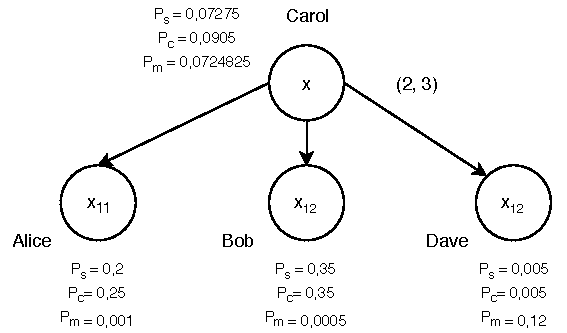
\includegraphics[width=0.6\linewidth]{images/chap_analisi_robustezza/robustezza-1.pdf}
\end{figure}

Concludiamo trovando $ R_c $ e $ R_s $.
\begin{tightcenter}
	$ R_c = 1 - 0,07275 = 0,92725 $\\
	$ R_s = 1 - 0,0905 - 0,0724825 = 0,8370175 $
\end{tightcenter}


\paragraph{Albero di distribuzione bilanciato di profondità 2}
Immaginiamo di avere a disposizione quattro agenti. Per tre di questi
vale
$ P_s = 0,1 $ \,
$ P_c = 0,3 $ \,
$ P_m = 0,02 $
mentre per il quarto abbiamo
$ P_s = 0,02 $ \,
$ P_c = 0,02 $ \,
$ P_m = 0,005 $.
Immaginiamo inoltre di utilizzare un albero di distribuzione simmetrico di profondità 2.
Come parametri per l'algoritmo di secret sharing usiamo $ t = 2 $ e $ n = 2 $ in tutti i casi.
La situazione è rappresentata in figura \ref{fig:robustezza-2-1}.

\begin{figure}[H]
	\centering
	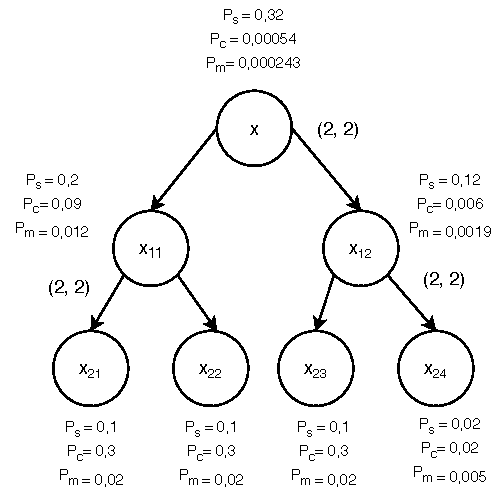
\includegraphics[width=0.6\linewidth]{images/chap_analisi_robustezza/robustezza-2-1.pdf}
	\caption{Albero di distribuzione bilanciato di profondità 2}
	\label{fig:robustezza-2-1}
\end{figure}

Calcoliamo gli attributi di $ x_{11} $. Abbiamo $ t = 2 $ e $ n = 2 $.
La resistenza agli smarimenti è $ \gamma = 0 $,
di conseguenza la $ P_s $ di $ x_{11} $ è data dalla somma delle $ P_s $ dei nodi figli.
$$ P_s = 0,1 + 0,1 = 0,2 $$

Per poter ottenere lo share $ x_{11} $ un attaccante esterno deve riuscire ad ottenere
sia $ x_{21} $ sia $ x_{22} $. Pertanto $ P_c $ è dato dal prodotto dei $ P_c $ dei nodi figli.
$$ P_c = 0,3 \cdot 0,3 = 0,09 $$

Se invece è uno degli agenti a voler ottenere $ x_{11} $  è sufficiente che ottenga
lo share dell'altro agente. Quindi $ P_m $ è data dalla somma delle probabilità
che si abbia sia un agente scorretto sia un agente corrotto.
$$ P_m = (0,02 \cdot 0,3) + (0,02 \cdot 0,3) = 0,0012 $$

Per quanto riguarda gli attributi di $ x_{12} $ abbiamo anche qui $ t = 2 $ e $ n = 2 $.
Il ragionamento è analogo a quello di cui sopra. Ci limitiamo
a riportare i calcoli.
\begin{tightcenter}
	$ P_s = 0,1 + 0,02 = 0,12 $      \\
	$ P_c = 0,3 \cdot 0,02 = 0,006 $ \\
	$ P_m = (0,02 \cdot 0,02) + (0,005 \cdot 0,3) = 0,0019 $
\end{tightcenter}
A questo punto dobbiamo trovare gli attributi di $ x $.
Si ha $ t = 2 $ e $ n = 2 $, anche qui il ragionamento è analogo a prima.
\begin{tightcenter}
	$ P_s = 0,2 + 0,12 = 0,32 $\\
	$ P_c = 0,09 \cdot 0,006 = 0,00054 $\\
	$ P_m = (0,012 \cdot 0,006) + (0,0019 \cdot 0,09) = 0,000243 $
\end{tightcenter}

Abbiamo quindi che
\begin{tightcenter}
	$ R_c = 1 - 0,32 = 0,68 $\\
	$ R_s = 1 - 0,00054 - 0,000243 = 0,999217 $
\end{tightcenter}

\paragraph{Albero di distribuzione con ridondanza}
Analogamente al caso precedente immaginiamo di avere a disposizione quattro agenti. Per tre di questi
vale
$ P_s = 0,1 $ \,
$ P_c = 0,3 $ \,
$ P_m = 0,02 $
mentre per il quarto abbiamo
$ P_s = 0,02 $ \,
$ P_c = 0,02 $ \,
$ P_m = 0,005 $.
Immaginiamo inoltre di utilizzare un albero di distribuzione simmetrico di profondità 2.
A differenza del caso precedente però utilizziamo $ t = 1 $ come threshold per gli share di secondo livello.
Facciamo notare che $ t = 1 $ significa che basta un solo share per ricostruire il messaggio originale,
ossia lo share è il messaggio originale. Di fatto possiamo vedere questa situazione come una
distribuzione degli share di primo livello ridondanti.
La situazione è rappresentata in figura \ref{fig:robustezza-2-2}.

\begin{figure}[H]
	\centering
	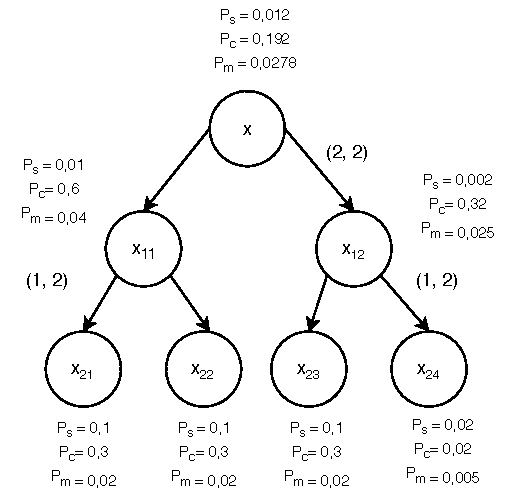
\includegraphics[width=0.6\linewidth]{images/chap_analisi_robustezza/robustezza-2-2.pdf}
	\caption{Albero di distribuzione con ridondanza}
	\label{fig:robustezza-2-2}
\end{figure}

Calcoliamo gli attributi di $ x_{11} $. Abbiamo $ t = 1 $ e $ n = 2 $.
Di fatto $ x_{11} $ è distribuito due volte, quindi
$ x_{11} $ viene smarrito se e solo se entrambi $ x_{21} $ e $ x_{22} $ vengono smarriti.
Di conseguenza per trovare
$ P_s $ dobbiamo moltiplicare i $ P_s $ dei nodi figli.
$$ P_s = 0,1 \cdot 0,1 = 0,01 $$


Per poter ottenere lo share $ x_{11} $ un attaccante esterno deve riuscire ad ottenere
o $ x_{21} $ o $ x_{22} $. Pertando $ P_c $ è dato dalla somma dei $ P_c $ dei nodi figli.
\begin{tightcenter}
	$ P_c = 0,3 + 0,3 = 0,6 $
\end{tightcenter}

Entrambi gli agenti di fatto conoscono $ x_{11} $, quindi per calcolare $ P_m $ si devono
sommare le $ P_m $ dei nodi figli.
\begin{tightcenter}
	$ P_m = 0,02 \cdot 0,02 = 0,04$
\end{tightcenter}

Per quanto riguarda gli attributi di $ x_{12} $ si ha $ t = 1 $ e $ n = 2 $,
i ragionamenti sono analoghi.
\begin{tightcenter}
	$ P_s = 0,1 \cdot 0,02 = 0,002 $\\
	$ P_c = 0,3 + 0,02 = 0,32 $\\
	$ P_m = 0,02 + 0,005 = 0,025 $
\end{tightcenter}

Non ci resta che trovare gli attributi di $ x $.
Abbiamo $ t = 2 $ e $ n = 2 $, il ragionamento è analogo a quello presente nell'esempio precedente.
\begin{tightcenter}
	$ P_s = 0,01 + 0,002 = 0,012 $\\
	$ P_c = 0,6 \cdot 0,32 = 0,192 $\\
	$ P_m = (0,04 \cdot 0,32) + (0,025 \cdot 0,6) = 0,0278 $\\
\end{tightcenter}

Troviamo infine che
\begin{tightcenter}
	$ R_c = 1 - 0,012 = 0.988 $\\
	$ R_s = 1 - 0,192 - 0,0278 = 0,7802 $
\end{tightcenter}

In questo caso siamo partiti avendo a disposizione gli stessi
agenti del caso precedente, ma utilizzando
un albero di distribuzione degli share differente abbiamo ottenuto risultati diversi.
Nello specifico, abbiamo migliorato la $ R_c $ ($ 0,988 $ contro $ 0,68 $), ma
allo stesso tempo abbiamo peggiorato la $ R_s $ ($ 0,7802 $ contro $ 0,999217 $).


\paragraph{Albero di distribuzione sbilanciato di profondità 2}
Ancora una volta immaginiamo di avere a disposizione quattro agenti. Per tre di questi
vale
$ P_s = 0,1 $ \,
$ P_c = 0,3 $ \,
$ P_m = 0,02 $
mentre per il quarto abbiamo
$ P_s = 0,02 $ \,
$ P_c = 0,02 $ \,
$ P_m = 0,005 $.
Questa volta però immaginiamo di utilizzare l'albero di distribuzione degli share
sbilanciato di profondità 2
mostrato in figura \ref{fig:robustezza-2-3}.
\begin{figure}[H]
	\centering
	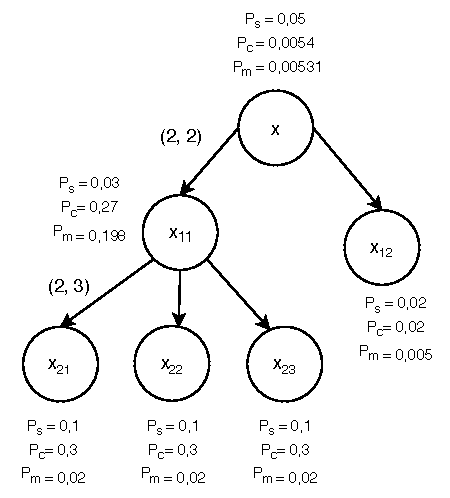
\includegraphics[width=0.6\linewidth]{images/chap_analisi_robustezza/robustezza-2-3.pdf}
	\caption{Albero di distribuzione sbilanciato di profondità 2}
	\label{fig:robustezza-2-3}
\end{figure}
Per prima cosa cerchiamo gli attributi di $ x_{11} $.
Abbiamo $ t = 2 $ e $ n = 3 $. La resistenza agli smarrimenti è $ \gamma = 1 $, perciò $ P_s $
è la somma delle probabilità delle tre combinazioni di avere $ \gamma + 1 = 2 $ smarrimenti.
\begin{tightcenter}
	$ P_s = (0,1 \cdot 0,1) + (0,1 \cdot 0,1) + (0,1 \cdot 0,1) = 0,03 $
\end{tightcenter}

La resistenza ai furti è $ \theta = 2 $. Un attaccante deve recuperare
due share per ottenere $ x_{11} $. Quindi
$ P_s = (0,3 \cdot 0,3) + (0,3 \cdot 0,3) + (0,3 \cdot 0,3) = 0,27 $

Infine $ P_m $ è
$$
	P_m = (0,02 \cdot 0,3) + (0,02 \cdot 0,3) +
	(0,02 \cdot 0,3) + (0,02 \cdot 0,3) +
	(0,02 \cdot 0,3) + (0,02 \cdot 0,3) = 0,198
$$
Non ci resta che trovare gli attributi di $ x $.
Ancora una volta $ t = 2 $ e $ n = 2 $.
\begin{tightcenter}
	$ P_s = 0,03 + 0,02 = 0,05 $      \\
	$ P_c = 0,27 \cdot 0,02 = 0,0054 $\\
	$ P_m = (0,198 \cdot 0,02) + (0,005 \cdot 0,27) = 0,00531 $
\end{tightcenter}

Troviamo infine che
\begin{tightcenter}
	$ R_c = 1 - 0,05 = 0,95 $\\
	$ R_s = 1 - 0,0054 - 0,00531 = 0,98929 $
\end{tightcenter}

Ancora una volta siamo partiti avendo a disposizione gli stessi
agenti dei casi precedenti. Con questa struttura di
albero di distribuzione degli share differente abbiamo ottenuto un risultato che
è un buon compromesso rispetto alle due soluzioni precedenti.
$ R_c $ è $ 0,95 $ contro gli $ 0,68 $ e $ 0.988 $ precedenti;
$ R_s $ è $ 0,98929 $ contro gli $ 0,999217 $ e $ 0,7802 $ precedenti.

In generale, non vi è un albero di distribuzione degli share ottimo; data una certa
situazione di agenti disponibili la progettazione dell'albero è il threshold su
cui possiamo agire per la determinazione delle performance del sistema.

\section{Considerazioni}
Questo modello può essere usato come un comodo strumento in grado di fornire
un'indicazione quantitativa sulla robustezza di una data implementazione.
Si tratta però di una approssimazione,
che non tiene conto di alcune dinamiche che si possono venire a creare. Infatti per poter
applicare questa tecnica di analisi si deve assumere che tutti gli agenti siano entità ben distinte
e che non vi siano coalizioni tra agenti. Inoltre è necessario attribuire a priori
$ P_s $, $ P_c $ e $ P_m $ ad ogni agente. Nella pratica questa è una attività non banale.

% In questo capitolo analizzeremo le principali criticità a cui il protocollo
% proposto è esposto. Per chiarezza di esposizione presenteremo
% i diversi scenari divisi per punti, ma è bene
% sapere che alcune di queste situazioni potrebbero verificarsi anche contemporanemente.

% \section{Comportamenti negligenti dei singoli utenti}
% \subsection{Uno o più agenti perdono il segreto}


% \subsection{L'agente si fa rubare il segreto}

% \subsection{Il client si fa rubare/pubblica il segreto prima di $ \tau $}


% \section{Comportamenti malevoli dei singoli utenti}
% \subsection{Comportamento malevole del client}

% \subsection{Comportamento malevolo di un agente}


% \section{Coalizioni tra agenti}


% \section{Un singolo attore controlla più agenti}
% DLT PERMISSIONED
% Affinché il protocollo funzioni al meglio
% è bene che tutti gli $ N $ agenti
% siano entità ben distinte. Purtroppo non in tutti i contesti
% questa caratteristica è facile da verificare.
% Possono quindi venirsi a creare situazioni nelle quali un unico soggetto controlla
% più agenti. Fissato $ k $ il numero di agenti che controlla,
% individuiamo due casi:
% \paragraph{Un singolo soggetto controlla $ k < \gamma $ agenti}
% In questo caso il soggetto non dispone di un numero sufficiente di share per
% ricostruire il segreto. Bisogna considerare però che parte da una posizione di
% vantaggio, perché deve recuperare solo altri $ \gamma - k $ share.
% \paragraph{Un singolo soggetto controlla $ k \geq \gamma $ agenti}
% In questo caso il soggetto dispone di un numero sufficiente di share per
% ricostruire il segreto. Significa che sin dal momento dell'inizializzazione
% del protocollo viene meno il requisito di
% segretezza del messaggio [vedi \ref{parag:segretezza-tre}].


% \section{Un soggetto corrompe gli agenti}
% Un attaccante che vuole ottenere il messaggio prima del tempo $ \tau $ deve riuscire
% ad ottenere almeno $ \gamma $ share.

% Un tecnica che può usare è quella di "corrompere" un numero $ \gamma $ di agenti.
% Per farlo deve offrire ad ogni agente una cifra maggiore di \textit{prize}.
% L'agente ha interesse nel tenere il proprio share segreto perché sa che se lo fa
% al tempo $ \tau $ può ottenere una ricompensa \textit{prize}.
% Se però un soggetto gli
% offre una cifra maggiore o uguale di \textit{prize} a quel punto l'azione
% più conviente diventa cedere il segreto.

% Come è possibile difendersi? Quello che può fare il client è fissare dei
% \textit{prize} adeguatamente alti rispetto al valore del segreto.
% Un'altra tecnica che può aiutare è quella di
% apportare un'ulteriore penalizzazione nel
% caso in cui l'agente ceda il segreto. Queste penalizzazioni possono essere
% legate al particolare dominio applicativo in cui il protocollo viene utilizzato.
% Un esempio è visibile nell'ultimo capitolo. TODO